\subsection{Effect of different cluster sizes}

\begin{figure}[H]
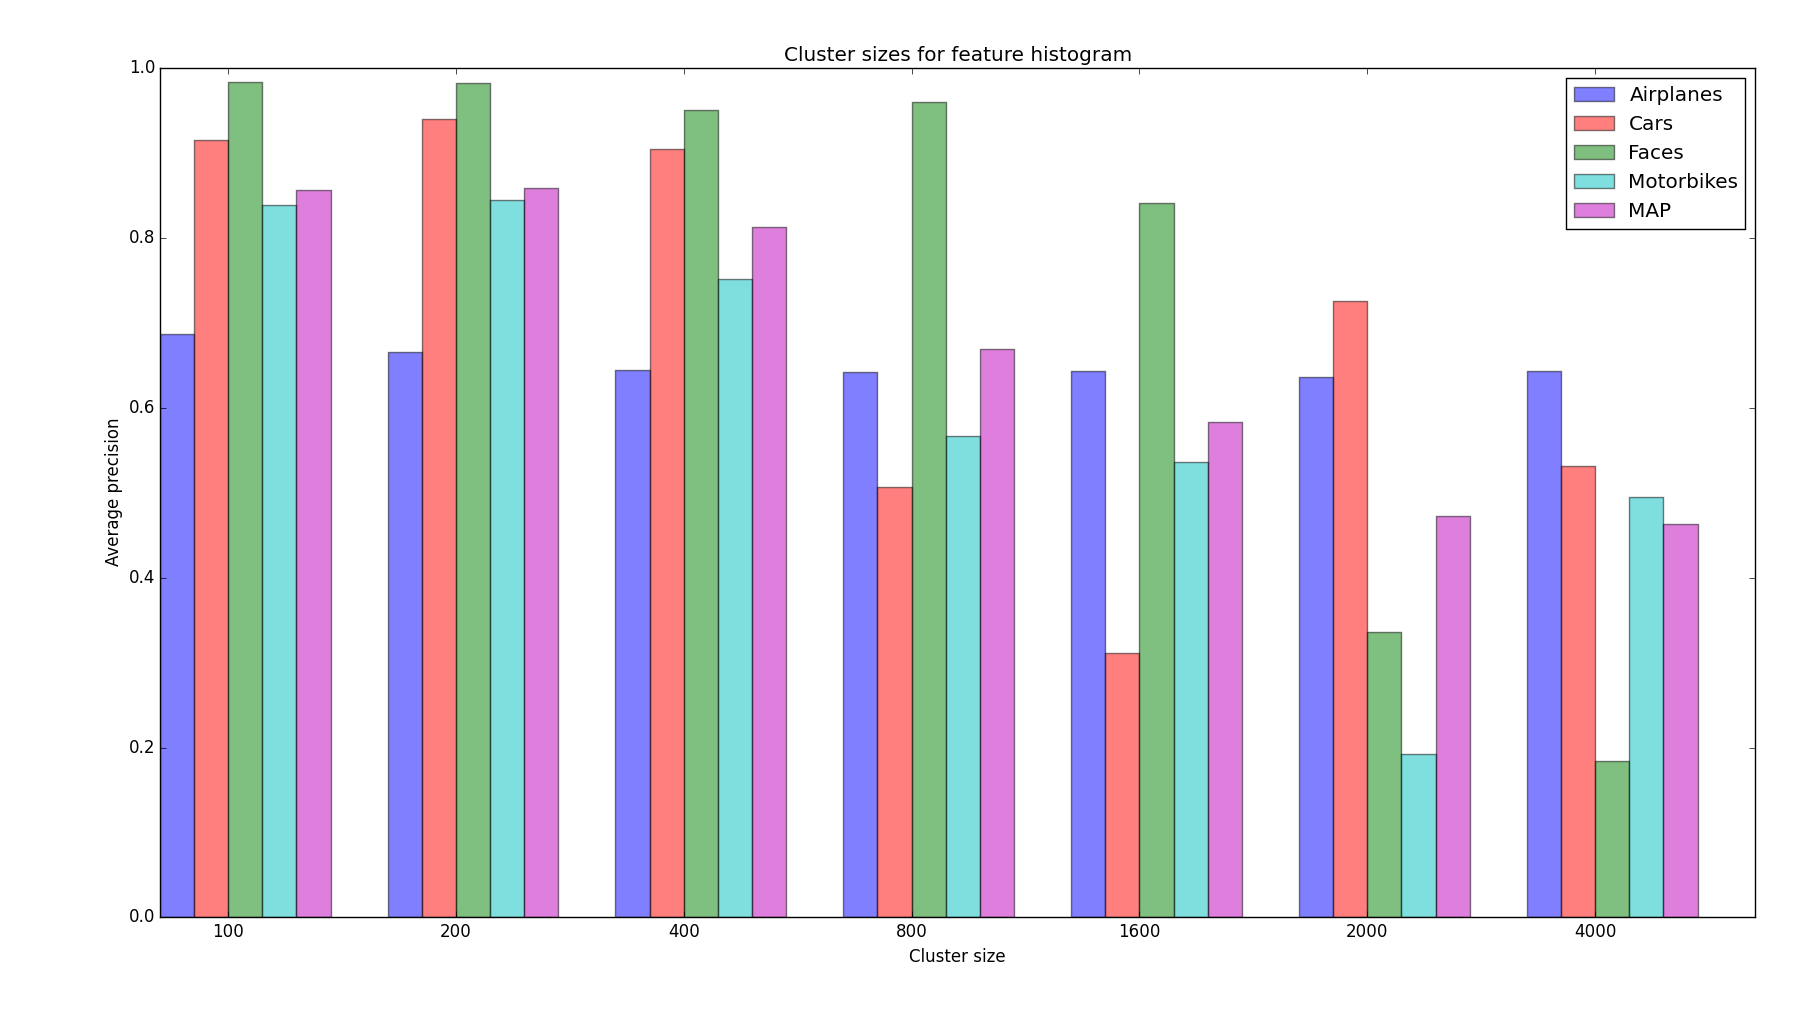
\includegraphics[width=\textwidth]{../plots/cluster_size_feature_histograms}
\caption{Effect of cluster size on AP}
\end{figure}
\begin{table}[H]
\begin{tabular}{|c|ccccc|}
\hline
\textbf{Cluster size} & \textbf{AP Airplanes} & \textbf{AP Cars} & \textbf{AP Faces} & \textbf{AP Motorbikes} & \textbf{MAP}\\
\hline
100& 0.6868 & 0.9152 & 0.9843 & 0.8395 & 0.8564\\
200 & 0.6663 & 0.9408 & 0.9824 & 0.8454 & 0.8587\\
400 & 0.6447 & 0.9053 & 0.9510 & 0.7516 & 0.8132\\
800 & 0.6424 & 0.5067 & 0.9602 & 0.5667 & 0.6690\\
1600 & 0.6438 & 0.3115 & 0.8410 & 0.5361 & 0.5831\\
2000 & 0.6367 & 0.7253 & 0.3357 & 0.1926 & 0.4726\\
4000 & 0.6430 & 0.5311 & 0.1837 & 0.4956 & 0.4634\\
\hline
\end{tabular}
\caption{Effect of different cluster sizes, Sift type: dense, Color space: opponent}
\label{tab:clusters}
\end{table}

The effect of changing the amount of clusters is shown in table \ref{tab:clusters}. In general, a smaller amount of clusters performs better than a large amount of clusters due to the data tending to overfit when a large amount of clusters is used. However, when a too small amount of clusters is used (e.g. 100), the amount of clusters is not capable of differentiating between different classes. The tipping point for the best performance regarding the amount of clusters is 200.